\documentclass{article}



%\usepackage{amssymb,latexsym,amsmath}
\usepackage{amssymb,latexsym}
%\usepackage{makeidx} 
%\makeindex

%\usepackage[dvips,matrix,arrow,ps,color,line,curve,frame]{xy}

%\usepackage{graphicx}

\usepackage[pdftex]{graphicx}

%\usepackage{parsetree}
\usepackage{hyperref}



\hoffset-0.64cm
\voffset-2.14cm


\textheight23.8cm

\setlength{\textwidth}{14.cm}



\begin{document}


\pagestyle{plain}










\newtheorem{theorem}{Theorem}[section]

\newtheorem{proposition}[theorem]{Proposition}

\newtheorem{lema}[theorem]{Lemma}

\newtheorem{corollary}[theorem]{Corollary}

\newtheorem{definition}[theorem]{Definition}

\newtheorem{remark}[theorem]{Remark}

\newtheorem{exempl}{Example}[section]

\newenvironment{example}{\begin{exempl}  \em}{\hfill $\square$

\end{exempl}}  \vspace{.5cm}









\renewcommand{\contentsname}{ }




\title{The EM rewrite system}

\author{Marius Buliga \\ 
\\
Institute of Mathematics, Romanian Academy \\
P.O. BOX 1-764, RO 014700\\
Bucure\c sti, Romania\\
{\footnotesize Marius.Buliga@imar.ro}}  \vspace{.5cm}







\date{This version: \today}






\maketitle


\begin{abstract}
We study emergent algebras as a term rewrite system. 

\end{abstract}


%\tableofcontents


%\newpage

\section{Finite terms}

Let $\Upsilon$ be a nonempty collection of node variables and $X$ a collection of edge variables. $\mathcal{C}$ is a collection of constant terms, which will be specified later. We have at our disposal an unspecified collection of names, in case we need them. All these collections are disjoint sets. 

The collection $\mathcal{C}$ contains at least four terms: $0$, $1$, $\displaystyle \bar{1}$ and $T$. The last one is called the terminator. 



\begin{definition}
Any finite term is obtained after a finite number of applications of the following rules:
\begin{enumerate}
\item[-] if $x \in X$ is an edge variable then $x$ is a term. $Nodevar(x)=\emptyset$ and $Edgevar(x)=\left\{ x \right\}$.
\item[-] if $x,y$ are terms and $a \in \Upsilon$ is a node variable then $\displaystyle a^{x}y$ and $\displaystyle \bar{a}^{x}y$  are terms. 
$$Nodevar\left( a^{x} y \right) = Nodevar\left( \bar{a}^{x} y \right) =  \left\{ a \right\} \cup Nodevar(x) \cup Nodevar(y)$$
$$Edgevar\left( a^{x} y \right) = Edgevarvar\left( \bar{a}^{x} y \right) = Edgevar(x) \cup Edgevar(y)$$
\item[-] any constant term is a term. 
\end{enumerate}

The arity of a term $x$ is the number of elements of $Edgevar(x)$. The terminator has arity 1, $0$ and $1$ have arity 2.

A node variable $a \in \Upsilon$ is fresh for a term $x$ if $\displaystyle a \not \in Nodevar(x)$. An edge variable $y \in X$ is fresh for a term  $x$  if 
$\displaystyle y \not \in Edgevar(x)$.

Two terms are equal "$x=y$" if they are identical up to alpha renaming of their node and edge variables. 
\label{defterms}
\end{definition}



We represent terms by their syntactic trees. A syntactic tree is a particular case of an oriented ribbon graph, where we assume that the edges of the syntactic tree are oriented from the leaves to the root and that any node of the syntactic tree has only one output edge and the order of the other edges comes from the clockwise orientation, starting from the output edge. We do not distinguish between terms and their graph representation. 





The following convention is used: we are free to define a term by giving it a name (which should not be a node or edge variable). Graphically a defined term appears as a node with the name of the term and a collection of half edges. If the term has arity $n$ then as a node in an oriented ribbon graph it will have $n+1$ half edges (except for the terminator), which can be uniquely identified by their  appearance in the clockwise order. The node variables of the term appear as decorations of the node. The input half edges are decorated with terms. (Some times we shall use another color, for example red, for the decorations of the leaves. Other times we shall just number the leaves, in the right order.) The root is left without any decoration (other than the terminator, perhaps). 

Whenever we draw syntactic trees, the root will appear at the left of the figure. In this way the orientations of the edges can be deduced from the rules from the clockwise order on the page, the position of the root and the color or names of the nodes. 

\vspace{.5cm} 
\centerline{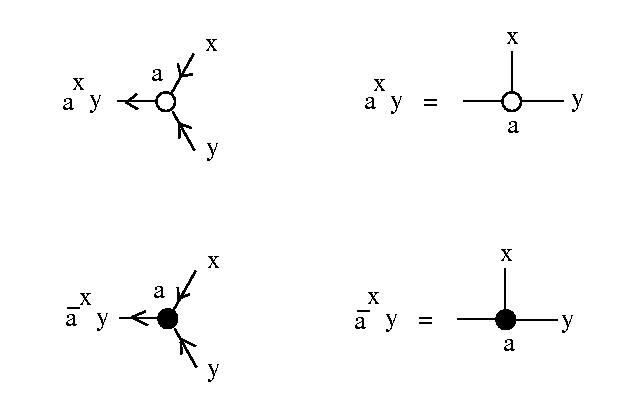
\includegraphics[width=80mm]{jpg/shuffle_00.jpg}} \vspace{.5cm} 

If $a \in \Upsilon$ and $x , y$ are terms then the term $\displaystyle a^{x}y$ appears as a white (or empty) circle, decorated with $a$, and the term $\displaystyle a^{x}y$ appears as a white (or empty) circle, decorated with $a$. 



A forrest of trees, with only one root which is not decorated by a terminator, counts for us as a term. 

The terminator is seen as a decoration of a root of a syntactic tree. The convention is to ignore any tree with the root decorated with a terminator. We need terminators only for technical purposes, like the need to be able to describe rewrites of the constants $0$ and $1$, or to be able to mark some terms for erasure, or for an implementation of a garbage collection algorithm, if needed. For this article the terminator is one of the mild inconveniences due to the fact that written articles are not programs, but any program which implements what is described in the article has to contain a terminator, which is moreover easy to build. On the other side, as articles, less rigorous as programs, are targeted for a human audience,  the concept of a terminator is very easy to grasp. 


 \vspace{.5cm}



Further is a list of terms which are going to be important in the exposition. 



\begin{definition}
If $a \in \Upsilon$ is a node variable and $b$ a binary term (i.e. it has arity 2) then $\displaystyle a-b$ is the term: 

\vspace{.5cm} 
\centerline{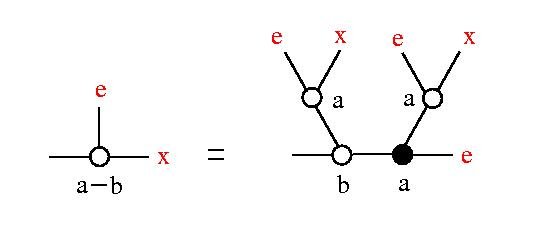
\includegraphics[width=80mm]{jpg/a-b.jpg}} \vspace{.5cm} 


If $a$ and $b$ are binary terms then $\displaystyle ab$ is the term: 

\vspace{.5cm} 
\centerline{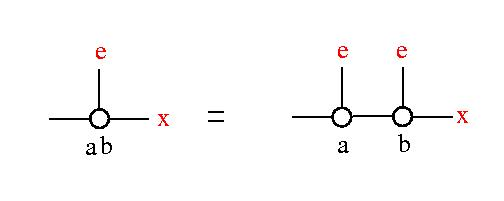
\includegraphics[width=70mm]{jpg/ab.jpg}} \vspace{.5cm} 

The constant terms $0$, $1$ and $\displaystyle \bar{1}$ have arity 2 and are defined via the terminator, as: 

\vspace{.5cm} 
\centerline{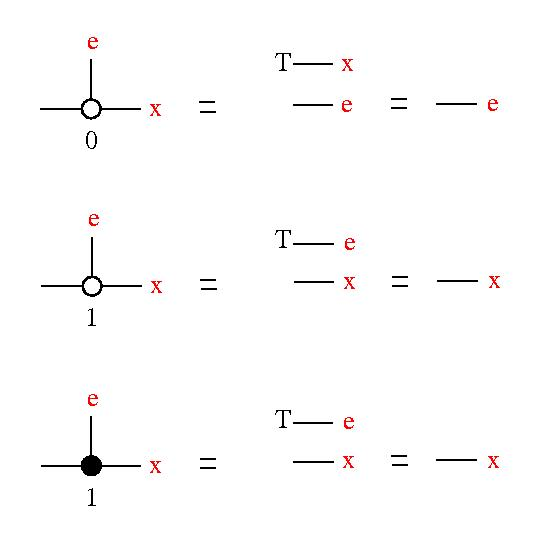
\includegraphics[width=70mm]{jpg/0.jpg}} \vspace{.5cm} 

\label{ddifprod}
\end{definition}


\section{Pattern matching equalities}
\label{spatmat}

For any node variables $a, b \in \Upsilon$ and $b, d$ terms, just by pattern matching, we have:  

\begin{figure}[h]
   \centerline{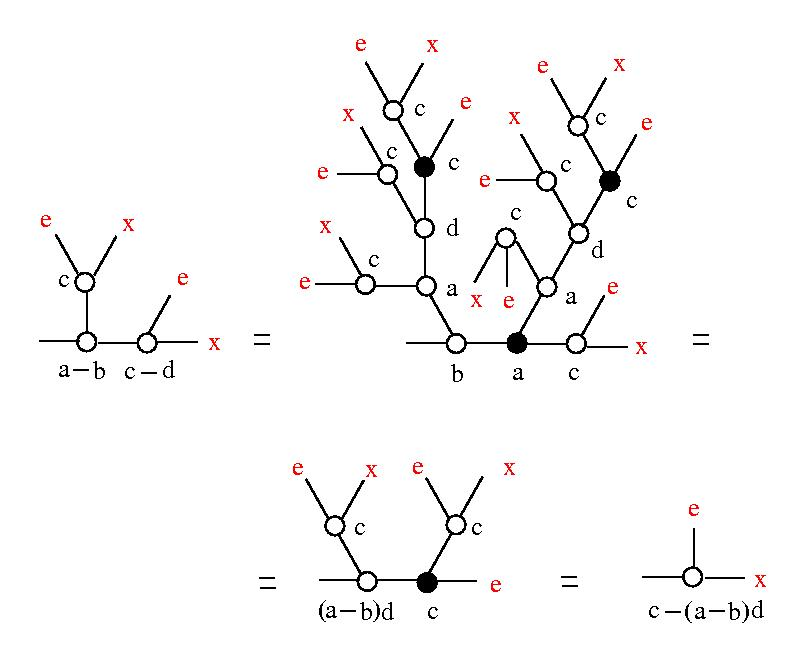
\includegraphics[width=100mm]{jpg/accept_4.jpg}}
\caption{ c-(a-b)d }
\label{fig1}
\end{figure}

Remark that the multiplication is obviously associative, i.e. $(ab)c = a(bc)$ for any terms $a, b, c$.



Let's see what this could mean. For expository purposes let's take $\Upsilon = (0,1)$ and the edge variables collection $X$ to be a real vector space. (As well we could take 
$$\displaystyle \Upsilon \, = \,  \left\{ a \in \mathbb{C}^{*} \mbox{ : } \mid a \mid < 1 \right\}$$ and $X$ a complex vector space. Later we shall see that these are only very particular examples of a general phenomenon.) Define further $\displaystyle a^{x}y = (1-a)x + ay$, or graphically: 
\vspace{.5cm} 
\centerline{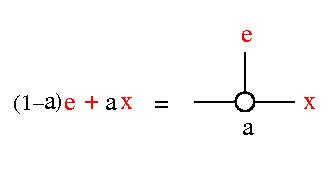
\includegraphics[width=50mm]{jpg/accept_0_1.jpg}} \vspace{.5cm}
and $\displaystyle \bar{a}=a^{-1}$. Then, for $a, b \in \Upsilon$ and $e, x \in X$ we have, by Definition \ref{ddifprod}
$$ (a-b)^{e} x \, = \,  b^{a^{e} x} \,  \bar{a}^{a^{e} x} e \, = \, (1-b) ((1-a) e + a x) + b ((1-a^{-1})((1-a)e + a x) + a^{-1}e) \, = \, $$ 
$$ = \, (1-b) ((1-a) e + a x) + b ((2-a)e + (a-1)x) \, = \, $$ $$ = \, ((1-b)(1-a) + b(2-a)) e + ((1-b)a + b(a-1))x \, = \, $$ 
$$ =\, (1-a+b)e + (a-b)x
$$ 
which motivates, in this very particular example, the reason behind the definition of the term $a-b$. A similar, but simpler computation for the product, is: 
$$(ab)^{e} x \, = \, a^{e} \, b^{e} x \, = \, (1-a) e + a((1-b)e + bx) \, = \, (1-ab)e + ab x$$
We can check that $$\displaystyle 0^{e} x \, = \, (1-0) e + 0 x = e$$  $$\displaystyle 1^{e} x \, = \, \bar{1}^{e} x \,  = \, (1-1)e + 1 x \, = \, x$$

The equality from the Figure (\ref{fig1}) where we used pattern matching is then (for $a, b, c, d \in \Upsilon$): 
$$ (a-b)^{c^{e} x} \, (c-d)^{e} x \, = \, (c-(a-b)d)^{e} x $$
which is indeed true, because
$$(a-b)^{c^{e} x} \, (c-d)^{e} x \, = \, (1-a+b) ((1-c) e + c x) + (a-b) ((1-c+d) e + (c-d)x) = \, $$ 
$$ = \, ((1-a+b)(1-c) + (a-b)(1-c+d)) e + ((1-a+b)c + (a-b)(c-d)) x \, = \,$$
$$ = \,  (1-c-a+ac+b-bc+a-b-ac+bc+ad-bd) e + (c-ac+bc+ac-bc-ad+bd)x \, = $$ 
$$ = \, (1-c+ad-bd) e + (c-ad+bd)x$$
and 
$\displaystyle (c-(a-b)d)^{e} x \, = \, = (c-ad+bd)^{e} x \, = \, (1-c+ad-bd) e + (c-ad+bd)x$. 

\vspace{.5cm}

\paragraph{Discussion.} We can prove (in Figure \ref{a-0-fig}) by pattern matching that, in general, for any $a \in \Upsilon$ 
\begin{figure}[h] \centerline{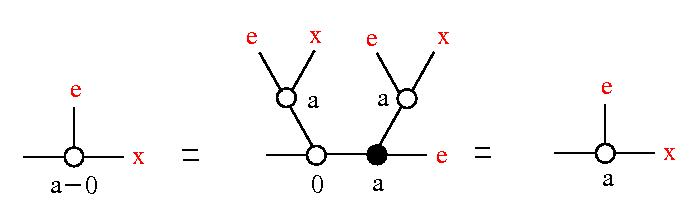
\includegraphics[width=110mm]{jpg/a-0.jpg}}  \caption{ $a-0 = a$ by pattern matching} \label{a-0-fig} \end{figure}
\begin{equation}
(a-0)^{e} x \,  = \, a^{e} x
\label{a-0}
\end{equation}
But we can't prove (in Figure \ref{a0-fig}) that  for any $a \in \Upsilon$ 
\begin{equation}
(a 0)^{e} x \,  = \, 0^{e} x \, = \, e
\label{a0}
\end{equation}
\begin{figure}[h] \centerline{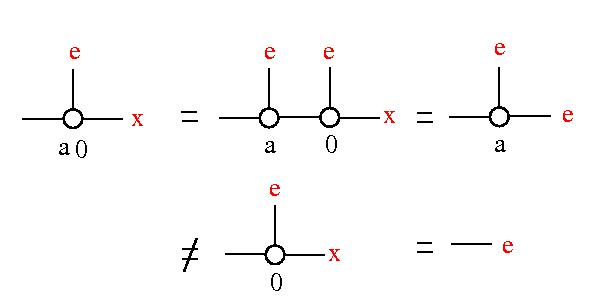
\includegraphics[width=100mm]{jpg/a0.jpg}}
\caption{ $a 0 \not = 0$ by pattern matching }
\label{a0-fig}
\end{figure}




In general, we can't prove by pattern matching only equalities like (\ref{a-a}) or (\ref{a-(a-b)}). 
\begin{equation}
(a-a)^{e} x \,  = \, 0^{e} x \, = \, e
\label{a-a}
\end{equation}

\begin{equation}
(a-(a-b))^{e} x \, =\, b^{e} x
\label{a-(a-b)}
\end{equation}
for any node variable $a \in \Upsilon$ and any binary term $b$.  

Indeed, Figure \ref{a-a-fig} shows this for (\ref{a-a}).  More interestingly, if we try to prove (\ref{a-(a-b)}) by pattern matching, like in Figure \ref{a-(a-b)-fig}, then at some point we are stuck without something like (\ref{a-a}) to use. 

\begin{figure}[h]\centerline{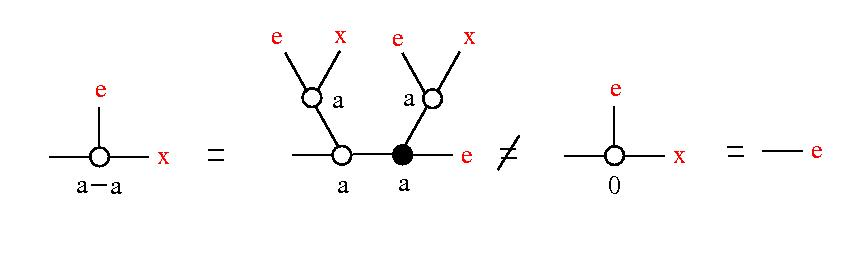
\includegraphics[width=120mm]{jpg/a-a.jpg}}  \caption{ $a-a \not = 0$ by pattern matching } \label{a-a-fig}  
\end{figure}

\begin{figure}[h]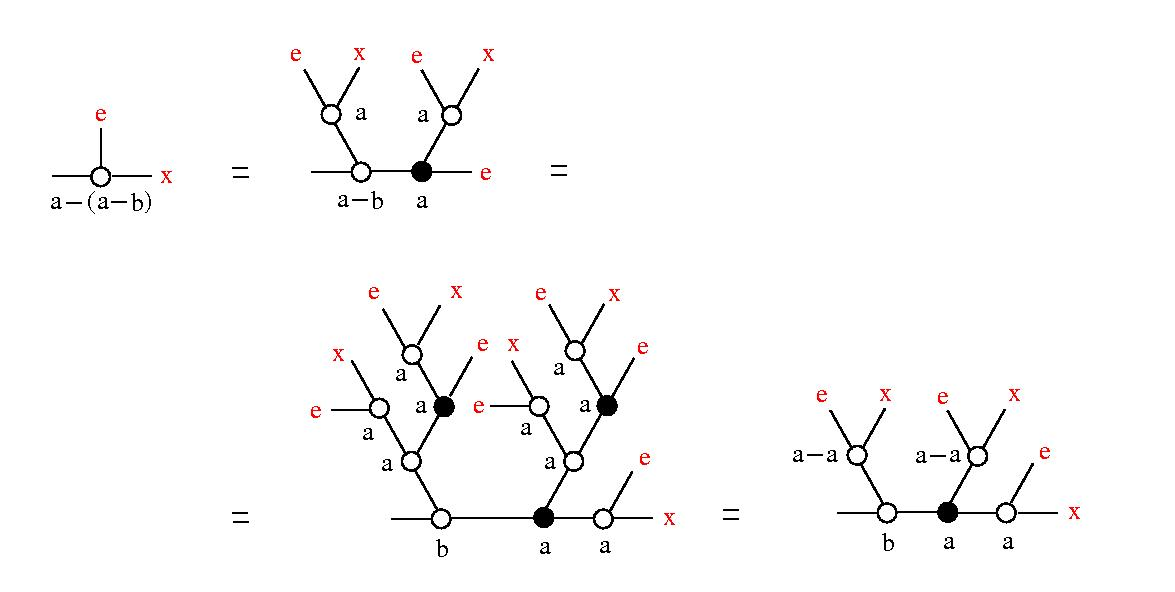
\includegraphics[width=120mm]{jpg/a-a-b.jpg}  \caption{ $a-(a-b) \not = b$ by pattern matching } \label{a-(a-b)-fig} \end{figure}




Another problem concerns the commutativity of multiplication. There is no reason for it in general. Remark for example that in Figure (\ref{fig1}) we wrote $(a-b)d$, where $a$ is a node variable and $b, d$ are terms. It is not true that $(a-b)d = d(a-b)$. The Figure \ref{a-bd-fig} shows that. 
\begin{figure}[h]\centerline{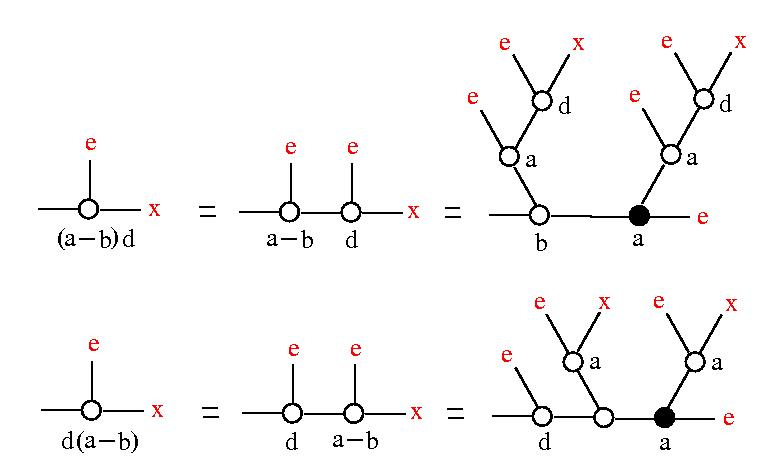
\includegraphics[width=100mm]{jpg/a-bd.jpg}}
\caption{ $(a-b)d \not = d(a-b)$ by pattern matching} \label{a-bd-fig} 
\end{figure}


Even for $a, b \in \Upsilon$ node variables, it is not true that 
\begin{equation}
(a b)^{e} x \, = (b a)^{e} x
\label{abba}
\end{equation}
\begin{equation}
(a \bar{b})^{e} x \, = (\bar{b}a)^{e} x
\label{abbara}
\end{equation}
\begin{equation}
(\bar{a} \bar{b})^{e} x \, = (\bar{b} \bar{a})^{e} x
\label{barabbara}
\end{equation}

With the choices made in the particular example, all  these equalities are trivially true and some of them are also equalities which we'd wish to have in general. But we don't have them by pattern matching only.


 
\section{Reidemeister 1, 2  rewrites}


We strengthen our formalism by the introduction of the Reidemeister 1 (Definition \ref{r1}) and Reidemeister 2 (Definition \ref{r2}) rewrites. We shall use the sign "$\displaystyle \longleftrightarrow$" for a rewrite, but also for any finite sequence of pattern matchings and rewrites. 

\begin{definition}
For any node variable $a \in \Upsilon$: 
\begin{enumerate}
\item[-] the first R1 rewrite is: $\displaystyle a^{x} x \, \longleftrightarrow \, x$
\item[-] the second R1 rewrite is:  $\displaystyle \bar{a}^{x} x \, \longleftrightarrow \, x$
\end{enumerate}
\centerline{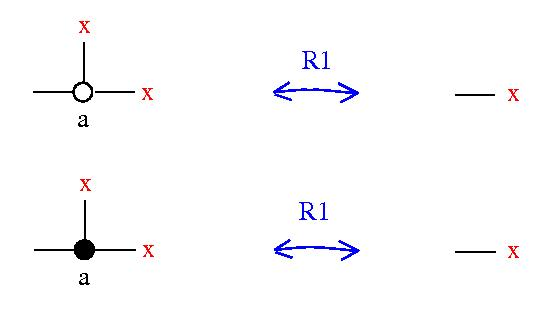
\includegraphics[width=80mm]{jpg/r1.jpg}}  
\label{r1}
\end{definition}



\begin{definition}
For any node variable $a \in \Upsilon$: 
\begin{enumerate}
\item[-] the first R2 rewrite is: $\displaystyle \left(\bar{a} a \right)^{e} x \, \longleftrightarrow \, x$
\item[-] the second R2 rewrite is:  $\displaystyle \left(a  \bar{a}\right)^{e} x \, \longleftrightarrow \, x$
\end{enumerate}
\centerline{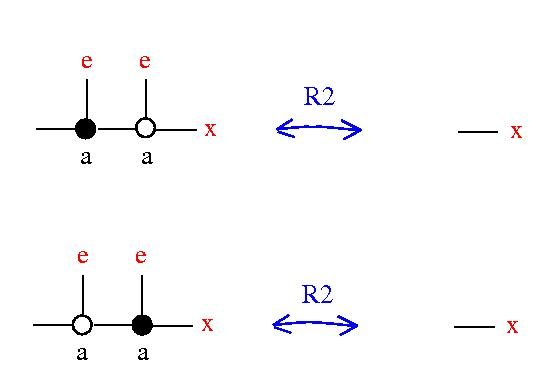
\includegraphics[width=80mm]{jpg/r2.jpg}}
\label{r2}
\end{definition}





\begin{proposition}
The first R1 rewrite is equivalent with the enforcing of the equation (\ref{a0}), in the sense that for any $a \in \Upsilon$ 
\begin{equation}
 (a 0)^{e} x \, \longleftrightarrow 0^{e} x 
\label{a01r1}
\end{equation}

The second R1 rewrite is equivalent with the first R1 rewrite and:  for any $a \in \Upsilon$ 
\begin{equation}
 ((a-1) 0)^{e} x \, \longleftrightarrow 0^{e} x 
\label{a02r1}
\end{equation}
\end{proposition}

 
\paragraph{Proof.} For the first R1 rewrite part the proof is  in the Figure \ref{a0r1-fig}. (This is almost similar with Figure \ref{a0-fig})
\begin{figure}[h]\centerline{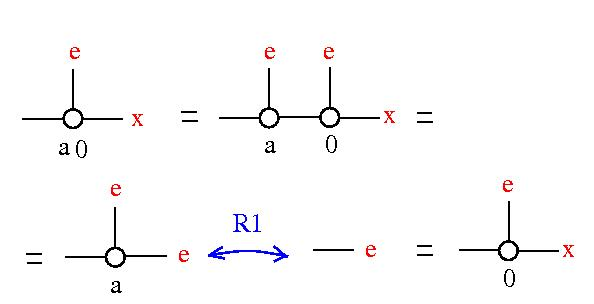
\includegraphics[width=80mm]{jpg/a0r1.jpg}}  \caption{ The first R1 rewrite is equivalent with $a 0 = 0$ } \label{a0r1-fig} \end{figure}
For the second R1 rewrite part see  the Figure \ref{a-1r1-fig}. 
\begin{figure}[h]\centerline{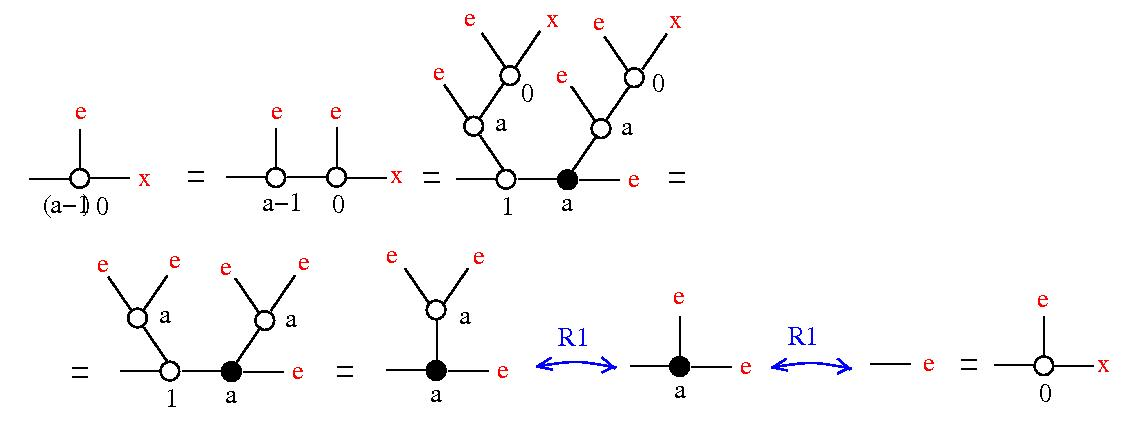
\includegraphics[width=120mm]{jpg/a-1r1.jpg}}  \caption{ The second R1 rewrite is equivalent with $(a-1) 0 = 0$ } \label{a-1r1-fig} \end{figure}

\vspace{.5cm}


The Reidemester 2 rewrites are related to pattern matching equalities (\ref{a-a}) and (\ref{a-(a-b)}),  from the Figures \ref{a-a-fig} and \ref{a-(a-b)-fig}.  

\begin{proposition}
The second R2 rewrite implies that for any $a \in \Upsilon$
\begin{equation} 
 (a - (a - 0))^{e} x \, \longleftrightarrow 0^{e} x 
\label{2r2}
\end{equation}
Conversely, (\ref{2r2}) implies that the first R2 rewrite is equivalent with: for any $a \in \Upsilon$
\begin{equation} 
 (a - (a - 1))^{e} x \, \longleftrightarrow 0^{e} x 
\label{1r2}
\end{equation}
\label{pr2}
\end{proposition}





\paragraph{Proof.} For the first implication see the Figure \ref{a-a-0r2-fig}. For the second implication see the Figure \ref{a-a-1r2-fig}. 
\begin{figure}[h]\centerline{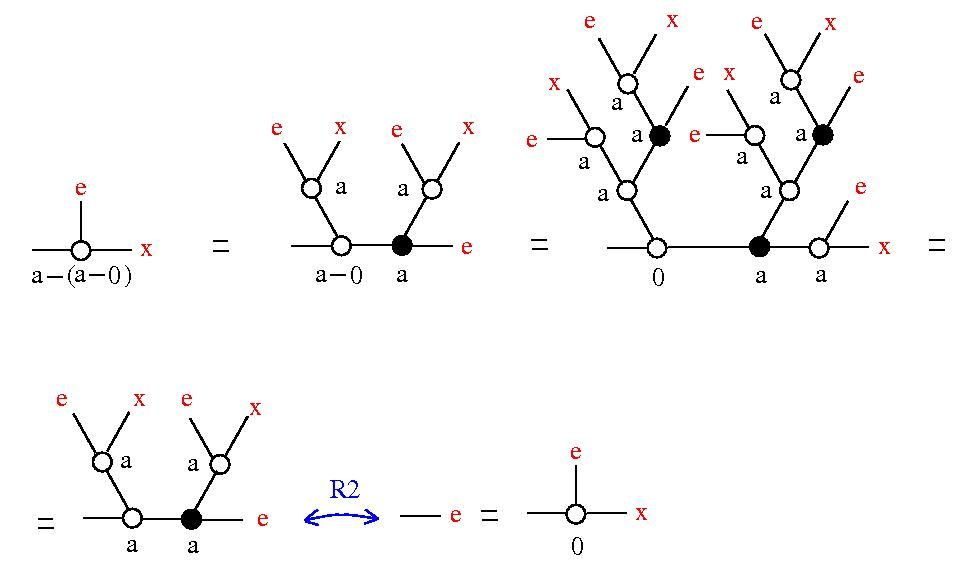
\includegraphics[width=120mm]{jpg/a-a-0r2.jpg}}  \caption{ The second R2 rewrite implies $a-(a-0) = 0$ } \label{a-a-0r2-fig} \end{figure}

\begin{figure}[h]\centerline{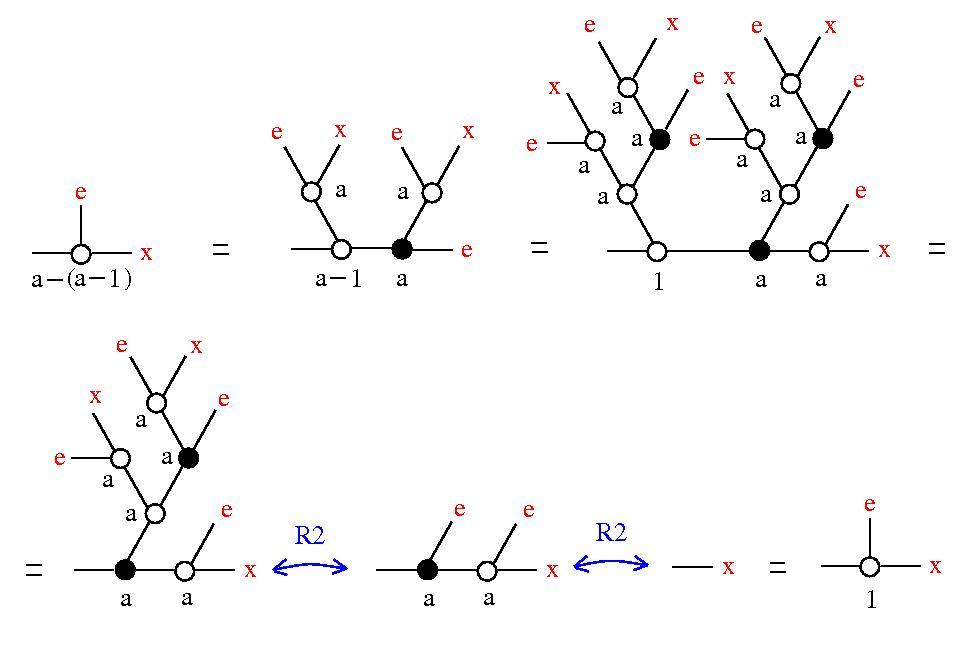
\includegraphics[width=120mm]{jpg/a-a-1r2.jpg}}  \caption{ The first R2 rewrite is equivalent with $a-(a-1) = 1$ } \label{a-a-1r2-fig} \end{figure}

\vspace{.5cm}



\section{Idempotent right quasigroups}

The connection between these rewrites and the true Reidemeister moves from knot theory is the following. Knot diagrams are ribbon graphs (oriented or not) made of two kinds of 4 valent nodes, which are also planar graphs (a condition which is irrelevant for this exposition) and the Reidemeister moves are indeed graph rewrites which apply on this class of graphs (planar or not). Knot diagrams (edges) can be decorated by elements from an algebraic structure called "quandle", in such a way that the Reidemeister rewrites (from knot theory) preserve the decoration. A quandle is a self-distributive idempotent right quasigroup and the correspondence between the Reidemeister rewrites (from knot theory) and the axioms of a quandle is the following: "self-distributive" = R3, "idempotent" = R1, "right quasigroup" = R2. For the convenience of the reader we give here the definition of an idempotent right quasigroup. 

\begin{definition}
An idempotent right quasigroup (irq) $\displaystyle (X, \circ, \bullet)$ is a set $X$ with two binary operations which satisfy the axioms: 
\begin{enumerate}
\item[-] (R1) for any $x \in X$ \, $\displaystyle x \circ x \, = x \bullet x \, = \, x$
\item[-] (R2) for any $e, x \in X$ \, $\displaystyle e \bullet ( e \circ x) \, = \, e \circ (e \bullet x) \, = \, x$
\end{enumerate}
\label{irq}
\end{definition}

A simple example of an irq is given by $\displaystyle (X, \circ_{a}, \bullet_{a})$, 
$$\displaystyle x \circ y \, = \, (1-a)x + ay \, , \, x \bullet y \, = \, (1-a^{-1})x + a^{-1}y $$
where $x, y \in X$, a real vector space and $a \in (0, + \infty)$ is a fixed parameter. (This example is actually a quandle, meaning that it satisfies also a third axiom R3 of self-distributivity). The calculations made at the beginning of Section \ref{spatmat} were done in this particular irq. 

If we consider instead a family of irqs indexed with a parameter $a \in Y$ then we arrive to the notion of a $Y$-irq, Definition 4.2 \cite{buligabraided}, or Definition 5.1 \cite{buligaglc}. In Definition 3.3. \cite{buligairq} we started from one irq and defined a $\mathbb{Z} \setminus \left\{ 0 \right\}$ -irq. 

\begin{definition}
Let $Y$ be a commutative group, with the operation denoted multiplicatively and the neutral element denoted by $1$. A $Y$-irq is a family of irqs $\displaystyle (X, \circ_{a}, \bullet_{a})$, for any $a \in Y$, with the properties: 
\begin{enumerate}
\item[-] (a) for any $x,y \in X$ \, $\displaystyle x \circ_{1} y \, = \, x \bullet_{1} y \, = \, y$
\item[-] (b) for any $a \in Y, \, x, y \in X$ \, $\displaystyle x \circ_{a^{-1}} y \, = \, x \bullet_{a} y$
\item[-] (c) for any $a, b \in Y, x, y \in X$ \, $x \circ_{a} ( x \circ_{b} y) \, = \, x \circ_{ab} y$.   
\end{enumerate}
\label{yirq}
\end{definition}

This definition has many points in common with parts of Definitions \ref{defterms}, \ref{ddifprod}, \ref{r1} and \ref{r2}. Here $X$ plays the role of the set of terms,  $\displaystyle \left\{ a, \, \bar{a} \mbox{ : } a \in \Upsilon\right\}$ plays the role of the group $Y$, $\displaystyle \longleftrightarrow$ plays the role of "$=$". If we replace "$\displaystyle a^{e} x$" by "$\displaystyle e \circ_{a} x$", and "$\displaystyle \bar{a}^{e} x$" by "$\displaystyle e \bullet_{a} x$" then: 
\begin{enumerate}
\item[-] Definition \ref{yirq} (a) corresponds to Definition \ref{ddifprod}, the part about $\displaystyle 1$ and $\displaystyle \bar{1}$, 
\item[-] Definition \ref{yirq} (b) corresponds to the choice of graphical notation for the terms $\displaystyle a^{e} x$ and $\displaystyle \bar{a}^{e} x$, 
\item[-] Definition \ref{yirq} (b) corresponds to Definition \ref{ddifprod} of multiplication of two binary terms.  
\item[-] $\displaystyle (X, \circ_{a}, \bullet_{a})$ is an irq corresponds to Definitions \ref{r1}, \ref{r2}.
\end{enumerate}
There is no commutative group structure though, which corresponds to the fact that equations like (\ref{abba}), (\ref{abbara}) (\ref{barabbara}) do not hold. That is why we introduce the commutativity rewrites.


\section{Commutativity rewrites}

\begin{definition}
For any node variables $a,b \in \Upsilon$: 
\begin{enumerate}
\item[-] the first C rewrite is: $\displaystyle \left(a b \right)^{e} x \, \longleftrightarrow \, \left(b a  \right)^{e} x$
\item[-] the second C rewrite is: $\displaystyle \left(\bar{a} \bar{b} \right)^{e} x \, \longleftrightarrow \, \left(\bar{b} \bar{a}  \right)^{e} x$
\item[-] the third C rewrite is: $\displaystyle \left(\bar{a} b \right)^{e} x \, \longleftrightarrow \, \left(b \bar{a}  \right)^{e} x$
\end{enumerate}
\centerline{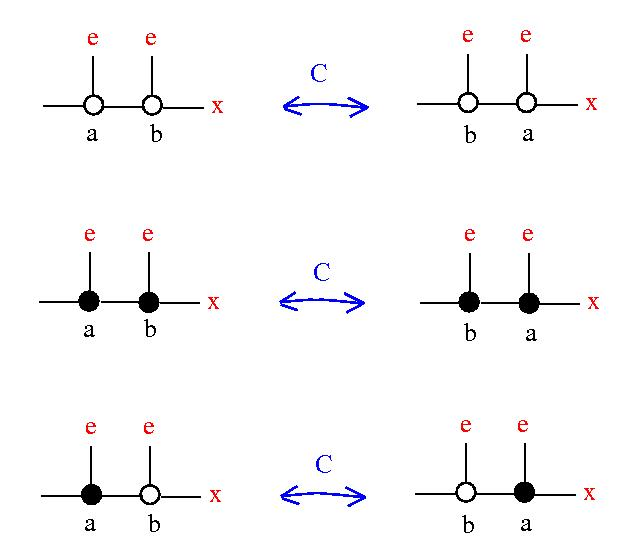
\includegraphics[width=80mm]{jpg/accept_3.jpg}}  
\label{c}
\end{definition}


\begin{proposition}
In the presence of the third C rewrite, the R2 rewrites are equivalent with: for any $a \in \Upsilon$ and any binary term $b$ 
\begin{equation}
 a - (a - b)^{e} x \, \longleftrightarrow \, b^{e} x 
\label{aab}
\end{equation}
\end{proposition}

\paragraph{Proof.} The third C rewrite can be used to show that the two R2 rewrites are equivalent. Use then Proposition \ref{pr2} to get that the two R2 rewrites are equivalent with 
(\ref{2r2}), (\ref{1r2}). Use the Figure \ref{a-(a-b)-fig} to deduce (\ref{aab}). Conversely, (\ref{aab}) applied for $b = 0$ gives (\ref{2r2}) and for $b = 1$ gives (\ref{1r2}). 


\vspace{.5cm} 



There is no meaning for $a-b$ when $a, b \in Y$, in the realm of $Y$-irqs. However, looking back to the simple example of a $(0, \infty)$-irq made from a real vector space, we saw that $a-b$ (from Definition 
\ref{ddifprod}) does mean what is expected. On the other side, there are far more examples of irqs where there is no clear correspondent for this "$a-b$" operation. 


\section{Binary terms, algebraic structure}

In the following proposition we collect what we know until now. 

\begin{proposition}
The following are true: 
\begin{enumerate}
\item[-] for any $a \in \Upsilon$  $\displaystyle (a - a)^{e} x \, \longleftrightarrow \, 0^{e} x$
\item[-] for any $a \in \Upsilon$ and $b$ binary term $\displaystyle \left(a - \left(a - b\right)\right)^{e} x \, \longleftrightarrow \, b^{e} x$
\item[-] for any $a \in \Upsilon$  $\displaystyle \left(a 0 \right)^{e} x \, \longleftrightarrow \, 0^{e} x$
\item[-] for any binary term $b$  $\displaystyle \left(b 1 \right)^{e} x \, \longleftrightarrow \, b^{e} x$
\item[-] for any binary term $b$  $\displaystyle \left(1 b \right)^{e} x \, \longleftrightarrow \, b^{e} x$
\item[-] for any binary term $b$  $\displaystyle \left(0 b \right)^{e} x \, \longleftrightarrow \, 0^{e} x$
\item[-] if $b$ is a binary term such that $\displaystyle  \left(b 0 \right)^{e} x \, \longleftrightarrow \, 0^{e} x$ then for any $a \in \Upsilon$ $\displaystyle \left(\left(a-b\right) 0 \right)^{e} x \, \longleftrightarrow \, 0^{e} x$
\item[-] if $b, c$ are binary term such that $\displaystyle  \left(b 0 \right)^{e} x \, \longleftrightarrow \, 0^{e} x$,  $\displaystyle  \left(c 0 \right)^{e} x \, \longleftrightarrow \, 0^{e} x$ then $\displaystyle  \left(\left(b c\right) 0 \right)^{e} x \, \longleftrightarrow \, 0^{e} x$ 
\item[-] for any $a,b \in \Upsilon$ $\displaystyle \left(a b \right)^{e} x \, \longleftrightarrow \, \left(b a  \right)^{e} x$
\item[-] for any $a,b \in \Upsilon$ $\displaystyle \left(\bar{a} \bar{b} \right)^{e} x \, \longleftrightarrow \, \left(\bar{b} \bar{a}  \right)^{e} x$
\item[-] for any $a,b \in \Upsilon$ $\displaystyle \left(\bar{a} b \right)^{e} x \, \longleftrightarrow \, \left(b \bar{a}  \right)^{e} x$
\item[-] for any $a \in \Upsilon$ $\displaystyle \left(\bar{a} a \right)^{e} x \, \longleftrightarrow \, 1^{e} x  \, \longleftrightarrow \, \left(a \bar{a}  \right)^{e} x$
\end{enumerate}

\end{proposition}

As a consequence we obtain: 

\begin{proposition}
The set $\displaystyle \bar{\Gamma}$ is a commutative monoid with the operation of multiplication, neutral element $1$ and equality relation $\longleftrightarrow$. The set $\Gamma$ is a commutative group, subset of the monoid  $\displaystyle \bar{\Gamma}$, with the inverse unary operation generated by $\displaystyle a^{-1} = \bar{a} \, \bar{a}^{-1} = a$, for any $a \in \Upsilon$, and $\displaystyle 1^{-1} = 1$. 

The set $B\Upsilon$ is a noncommutative monoid with multiplication, neutral element $1$ and equality relation $\longleftrightarrow$. Moreover, for any $b, c \in B\Upsilon$ and for any $a \in \Upsilon$
\begin{enumerate}
\item[-] $a-b \in B\Upsilon$
\item[-] $0b \longleftrightarrow 0 \longleftrightarrow b0$ (i.e. $0$ is an absolute of the monoid $B\Upsilon$)
\item[-] $a-(a-b) \longleftrightarrow b$
\item[-] $a-0 \longleftrightarrow a$
\item[-] $\displaystyle a-1 \longleftrightarrow inv_{a}$ (see Definition \ref{aterms})
\end{enumerate}
\end{proposition}


\section{Approximate operations terms}

We introduce some new terms: aproximate sum, difference and inverse. The names come from dilation structures, Definition 11 \cite{buligadil1},  where they play an important role. 



\begin{definition}
The asum (approximate sum), adif (approximate difference) and ainv (approximate inverse) are the terms: 
\begin{enumerate}
\item[-] asum or approximate sum, for $a \in \Upsilon$: $\displaystyle \Sigma_{a}^{e}(x,y) \, = \, \bar{a}^{e} a^{a^{e} x} y$

\centerline{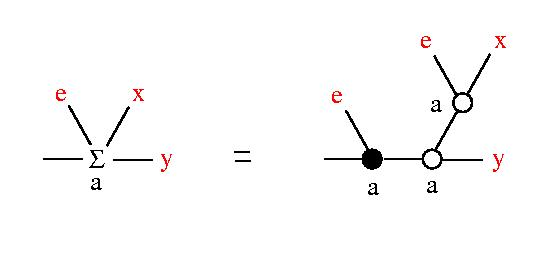
\includegraphics[width=80mm]{jpg/asum.jpg}}  
\item[-] adif or approximate difference, for $a \in \Upsilon$: $\displaystyle \Delta_{a}^{e}(x,y) \, = \, \bar{a}^{a^{e} x} a^{e} y$

\centerline{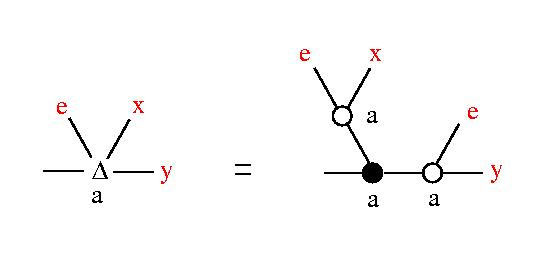
\includegraphics[width=80mm]{jpg/adif.jpg}}  
\item[-] ainv or approximate inverse, for $a \in \Upsilon$: $\displaystyle inv_{a}^{e} x \, = \, \bar{a}^{a^{e} x} e$

\centerline{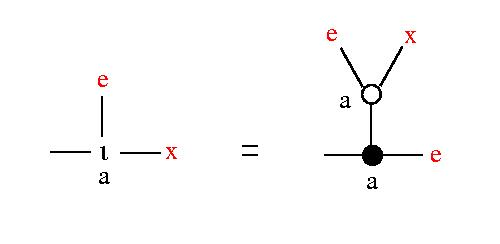
\includegraphics[width=80mm]{jpg/ainv.jpg}}  
\end{enumerate}
\label{aterms}
\end{definition}

We should think about the adif $\displaystyle \Delta_{a}^{e}(x,y)$ as the approximate difference of the vectors $-(e,x)+(e,y)$, based at $e$, and similarly about the asum or ainv. This is not needed in this general setting, but it is a good guide for the intuition of the reader. 

This analogy can be used to clarify the difference between the substraction $a - b$, with $a$ a node variable and $b$ a binary term, and the adif. We saw that, in the frame of real vector spaces and their associated irqs,  moreover with $e=0$ (the null vector of the vector space) for simplicity, 
$$\displaystyle (a-b)^{e} x \mbox{  is like }   (a-b)x$$
 In the same frame  
$$\displaystyle \Delta_{a}^{e}(x,y) \mbox{ is like } -(1-a)x + y$$
which is approximately $\displaystyle -x+y = y-x$. 

These asum, adif, ainv give to the terms a structure of an approximate conical group \cite{buligainf}, which can be informally described as an (approximate) non-commutative vector space. 
More precisely, by using the rewrites we have at our disposal, we can prove that the terms asum, adif, seen as binary operations, and ainv, seen as an unary operation, satisfy relations akin to associativity of the (vector) addition, the adif is an inverse to asum just like difference is the inverse of the sum, etc. These has been proved as identities several times, the ones we may need in this article are collected, for example, in Proposition 4.3 (a)--(g) \cite{buligabraided}, first time proved in Section 4.2  Definition 11 \cite{buligadil1}. 

As an example, the approximate associativity of asum is the statement: for any $a \in \Upsilon$ 
$$ \Sigma_{a}^{e}\left( \Sigma_{a}^{e}\left(x,y\right), z\right) \, \longleftrightarrow \, \Sigma_{a}^{e}\left( x, \Sigma_{a}^{a^{e} x} \left( y,z\right)\right) $$
whose proof is given in the Figure \ref{sumassoc}. 
\begin{figure}[h]\centerline{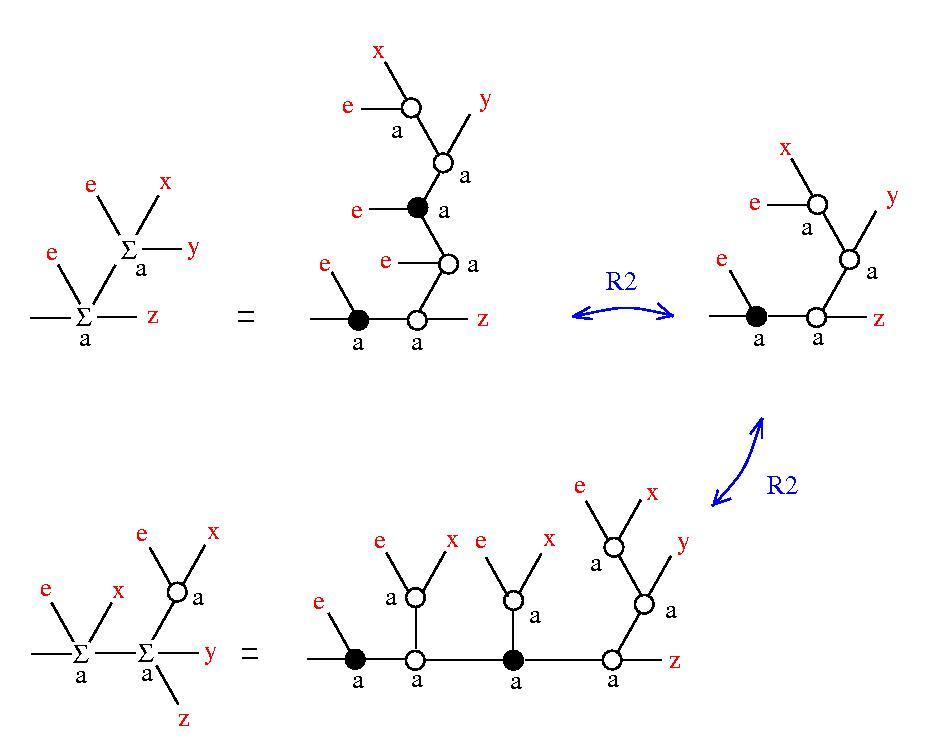
\includegraphics[width=120mm]{jpg/sumassoc.jpg}}  \caption{ The associativity of asum } \label{sumassoc} \end{figure}


\section{Limterms, LIM rewrites}
\label{emr}


The main idea of emergent algebras  is to allow the "passage to the limit" of the node variables, in some cases. This requires the enlargement of the class of constant terms, and the introduction of limterms. 

\begin{definition}
We add to the class of constant terms the ("exact") sum $\displaystyle \Sigma_{0}$,  the ("exact") diff $\displaystyle \Delta_{0}$, the ("exact") inv $\displaystyle inv_{0}$. 

We define the class of limterms as: 
\begin{enumerate}
\item[-] any term is a limterm. If $b$ is a term then the set of free node variables of $b$ is defined by $\displaystyle Freenodevar(b) \, = \, Nodevar(b)$ and the set of bonded node variables is  $Bondnodevar(b) \, = \, \emptyset$.
\item[-] if $a \in \Upsilon$ and $b$ is a limterm  then $\displaystyle L a. b$ is a limterm, with $\displaystyle Freenodevar(La.b) \, = \, Freenodevar(b) \setminus \left\{ a \right\}$ and $Bondnodevar(La.b) \, = \, Bondnodevar(b) \cup \left\{ a \right\}$.
\item[-] if $t$ is a limterm and $\displaystyle \in \Upsilon \cup \left\{ 0,1 \right\}$ then $t b$ is a limterm, with $\displaystyle Freenodevar(t b) \, = \, Freenodevar(t)$ and $\displaystyle Bondnodevar(t b) \, = \, Bondnodevar(t)$. 

The alpha renaming is extended to limterms. 
\end{enumerate}
\end{definition}

\begin{figure}[h]\centerline{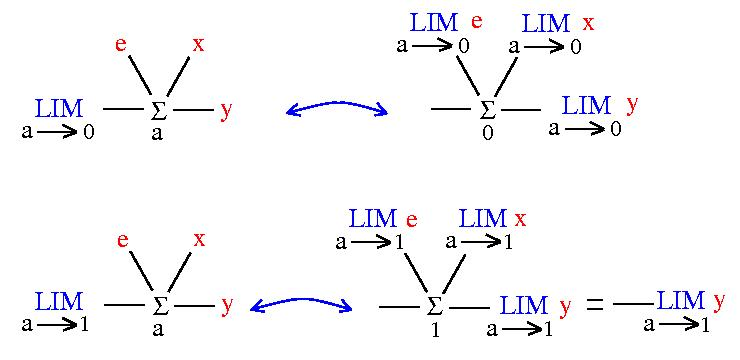
\includegraphics[width=120mm]{jpg/asum-em-alt.jpg}}  \caption{ The graphical notation for the LIM rewrite for the sum term} \label{asum-em-alt-fig} \end{figure}

\begin{definition}
The LIM rewrites are: 
\begin{enumerate}
\item[-] the LIM rewrites for edge variables: if $e$ is an edge variable, $a \in \Upsilon$ and $\displaystyle b \in \Upsilon \cup \left\{ 0 , 1 \right\}$, then $$(La.e)b \, \stackrel{LIM}{\longleftrightarrow} \, e$$  
\item[-] the LIM rewrites for node variable limterms: if $e, x$ are limterms then 
$$\displaystyle \left(La.\left(a^{e} x\right)\right) b  \, \stackrel{LIM}{\longleftrightarrow} \, b^{(La.e)b} (La.x)b$$ for $\displaystyle b \in \Upsilon \cup \left\{ 0 , 1 \right\}$, and  
$$\displaystyle \left(La.\left(\bar{a}^{e} x\right)\right) b  \, \stackrel{LIM}{\longleftrightarrow} \, \bar{b}^{(La.e)b} (La.x)b$$ for $\displaystyle b \in \Upsilon \cup \left\{  1 \right\}$. 
\item[-] the LIM rewrite for the sum term: if $e, x, y$ are limterms then 
$$\displaystyle \left( La.\Sigma_{a}^{e}(x,y) \right) b \, \stackrel{LIM}{\longleftrightarrow} \, \Sigma_{b}^{(La.e)b}((La.x)b,(La.y)b)$$ for $\displaystyle b \in \Upsilon \cup \left\{ 0 , 1 \right\}$. 
The term $\displaystyle \Sigma_{1}^{e} (x,y) \, = \, y$ is obtained from the application of the LIM rewrites for node variable terms to the limterm $\displaystyle (La.\Sigma_{a}^{e}(x,y)) 1$. 
\item[-] the LIM rewrite for the diff term: if $e, x, y$ are limterms then $$\displaystyle \left( La.\Delta_{a}^{e}(x,y)\right)b \, \stackrel{LIM}{\longleftrightarrow} \, \Delta_{b}^{(La.e)b}((La.x)b,(La.y)b)$$ for $\displaystyle b \in \Upsilon \cup \left\{ 0 , 1 \right\}$. 
The term $\displaystyle \Delta_{1}^{e} (x,y) \, = \, y$ is obtained from the application of the LIM rewrites for node variable terms to the term $\displaystyle (La.\Delta_{a}^{e}(x,y)) 1$. 
\item[-] the LIM rewrite for the inv term: $$\displaystyle \left(La.inv_{a}^{e} x\right) \, \stackrel{LIM}{\longleftrightarrow} \, inv_{0}^{(La.e)b} (La.x)b$$ for $\displaystyle b \in \Upsilon \cup \left\{ 0 , 1 \right\}$. The term $\displaystyle inv_{1}^{e} x  \, = \, e$ is obtained from the application of the LIM rewrites for node variable terms to the limterm $\displaystyle (La,inv_{a}^{e} x) 1$. 
\end{enumerate}

\end{definition}


\section{The EM meta-rewrite}

\begin{definition}
The EM meta-rewrite is: If $b, c$ are terms such that $\displaystyle b \leftrightarrow c$  and $\displaystyle d \in \Upsilon \cup \left\{ 0 , 1 \right\}$ then 
$$\displaystyle (La.b) d \stackrel{EM}{\longleftrightarrow} (La.c) d$$
An emergent rewrite is any chain $a \longleftrightarrow b$ of rewrites, where $a, b$ are terms and the chain contains at least a EM meta-rewrite. 
\end{definition}



\begin{figure}[h]\centerline{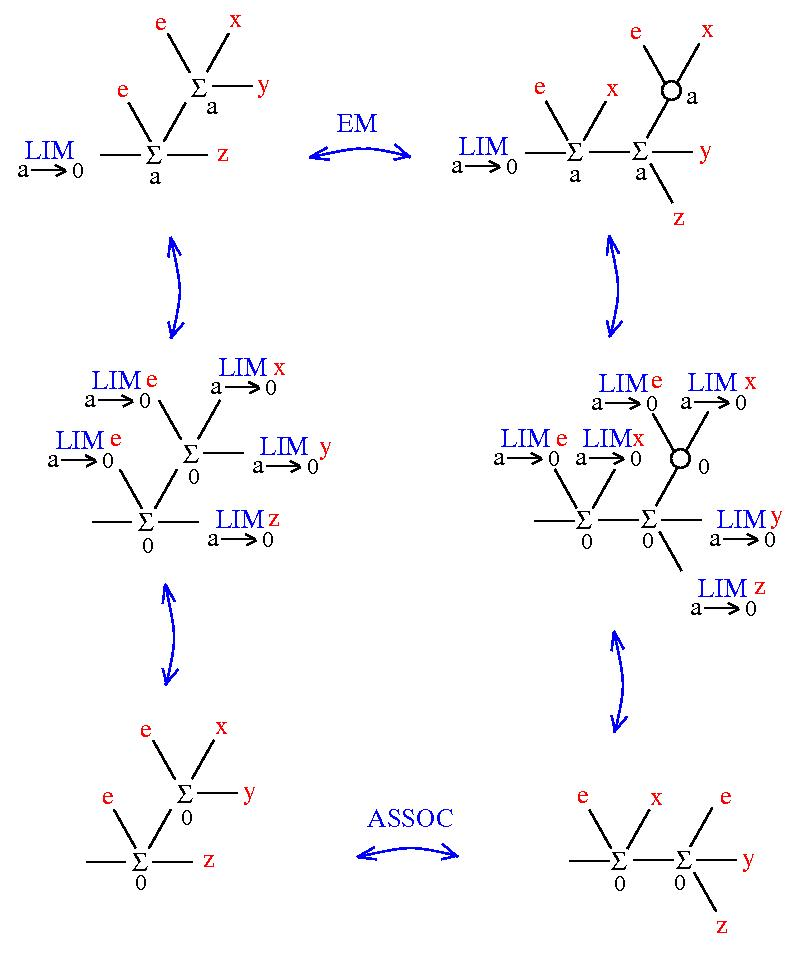
\includegraphics[width=120mm]{jpg/sumassoc-em.jpg}}  \caption{ The ASSOC rewrite is emergent. The EM meta-rewrite is applied for the rewrite from the Figure \ref{sumassoc}} \label{sumassoc-em-fig} \end{figure}

An example of an emergent rewrite is ASSOC, described in the Figure \ref{sumassoc-em-fig}. We use the Figure \ref{sumassoc} and we apply the EM meta-rewrite: for $e, x, y, z$ terms 
$$ \displaystyle \left(La.\Sigma_{a}^{e}\left( \Sigma_{a}^{e}\left(x,y\right), z\right)\right) 0 \, \stackrel{EM}{\longleftrightarrow} \, \left(La.\Sigma_{a}^{e}\left( x, \Sigma_{a}^{a^{e} x} \left( y,z\right)\right)\right) 0 $$
The limterm from the left hand side reduces, via LIM rewrites, as described in the left column of the Figure \ref{sumassoc-em-fig}: 
$$ \displaystyle \left(La.\Sigma_{a}^{e}\left( \Sigma_{a}^{e}\left(x,y\right), z\right)\right) 0 \, \stackrel{LIM}{\longleftrightarrow} \, $$ 
$$ \Sigma_{0}^{(La.e)0}\left( \left( La.\Sigma_{a}^{e}\left(x,y\right)\right) 0, (La.z)0\right) \, \stackrel{LIM}{\longleftrightarrow} \, $$ 
$$\Sigma_{0}^{e}\left( \Sigma_{0}^{(La.e) 0}\left((La.x)0,(La.y)0\right), z\right) \, \stackrel{LIM}{\longleftrightarrow} \, \Sigma_{0}^{e}\left( \Sigma_{0}^{e}\left(x,y\right), z\right)$$
In all detail there were 7 LIM rewrites and the last expression is a term. The limterm from the right hand side reduces in a slightly longer way: 
$$ \displaystyle  \left(La.\Sigma_{a}^{e}\left( x, \Sigma{a}^{a^{e} x} \left( y,z\right)\right)\right) 0 \, \stackrel{LIM}{\longleftrightarrow} \, $$ 
$$\Sigma_{0}^{(La.e) 0}\left( (La.x)0, La.\left(\Sigma_{a}^{a^{e} x} \left( y,z\right)\right) 0\right) \, \stackrel{LIM}{\longleftrightarrow} \, $$ 
$$ \Sigma_{0}^{e}\left( x , \Sigma_{0}^{\left(La.a^{e} x\right) 0} \left( (La.y) 0, (La.z) 0\right)\right) \, \stackrel{LIM}{\longleftrightarrow} \, $$
$$ \Sigma_{0}^{e}\left( x , \Sigma_{0}^{0^{(La.e) 0} (La.x) 0} \left( y, z\right)\right) \, \stackrel{LIM}{\longleftrightarrow} \, $$
$$ \Sigma_{0}^{e}\left( x , \Sigma_{0}^{0^{e} x} \left( y, z\right)\right) \, = \, \Sigma_{0}^{e}\left( x , \Sigma_{0}^{e} \left( y, z\right)\right)   $$
In this case there were 9 LIM rewrites until we obtain a term, then we use the definition of the term $0$ at the end.

We obtain the emergent rewrite: 
$$\Sigma_{0}^{e}\left( \Sigma_{0}^{e}\left(x,y\right), z\right) \, \stackrel{ASSOC}{\longleftrightarrow} \, \Sigma_{0}^{e}\left( x , \Sigma_{0}^{e} \left( y, z\right)\right)   $$
which expresses, in abstract syntactic tree (AST) form, the fact that for any term $e$ the operation $\displaystyle \Sigma_{0}^{e}(\cdot, \cdot)$ is associative. Mind that the operation itself is emergent: for any $e, x, y$ terms 
$$(\left(La. \Sigma_{a}^{e}(x,y)\right) 0  \, \stackrel{LIM}{\longleftrightarrow} \, \Sigma_{0}^{(La.e) 0} \left((La.x) 0 , (La.y) 0) \right)  \, \stackrel{LIM}{\longleftrightarrow} \, \Sigma_{0}^{e}(x,y)$$
Therefore, we are able to obtain emergent algebraic structures (operations) and properties of those (like associativity here) from the LIM rewrites of limterms, on one side, and from the use of the EM meta-rewrite with term rewrites, on the other side. 



%\section{Decorated tangles}

Recall that to any knot diagram is associated a quandle (which is an invariant, in the sense that the same quandle is associated to any other knot diagram obtained from a sequence of applications of R1, R1, R2 knot theory Reidemeister rewrites). We may consider knot diagrams with the crossings decorated with elements from a set $\Upsilon$, as explained in sections 3.3, 3.4 \cite{buligachora}.




\begin{thebibliography}{99}


\bibitem{buligaglc} M. Buliga, Graphic lambda calculus. {\it Complex Systems} {\bf 22}, 4 (2013), 311-360. \\ 
\href{https://arxiv.org/abs/1305.5786}{arXiv:1305.5786}

\bibitem{buligairq} M. Buliga, Emergent algebras, \href{https://arxiv.org/abs/0907.1520}{arXiv:0907.1520}

\bibitem{buligadil1} M. Buliga, Dilatation structures I. Fundamentals, {\it 
J. Gen. Lie Theory Appl.},  {\bf 1} (2007),  2, 65-95. \\ 
\href{https://arxiv.org/abs/math/0608536}{arXiv:math/0608536}


\bibitem{buligainf} M, Buliga, Infinitesimal affine geometry of metric spaces endowed with a dilatation structure, {\it Houston Journal of Mathematics}, {\bf 36}, 1 (2010), 91-136. \\ 
\href{https://arxiv.org/abs/0804.0135}{arXiv:math/0608536}


\bibitem{buligabraided} M. Buliga, Braided spaces with dilations and sub-riemannian symmetric spaces, in: Geometry. Exploratory Workshop on Differential Geometry and its Applications, eds. D. Andrica, S. Moroianu, Cluj-Napoca 2011, 21-35. \\   
\href{https://arxiv.org/abs/1005.5031}{arXiv:0804.0135}


\bibitem{buligachora} M. Buliga, Computing with space: a tangle formalism for chora and difference, \href{https://arxiv.org/abs/1103.6007}{arXiv:1103.6007}




%\bibitem{polyak} M. Polyak,  Minimal generating sets of Reidemeister moves,  \href{http://arxiv.org/abs/0908.3127}{arXiv:0908.3127}

%\bibitem{lodayr} J.-L. Loday, M.O. Ronco, Hopf Algebra of the  planar  Binary Trees, {\it Advances in Math.}, {\bf 139} (1998), 293-309

\bibitem{graphiclambdaknots} M. Buliga, Graphic lambda calculus and knot diagrams, \href{http://arxiv.org/abs/1211.1604}{arXiv:1211.1604}


\bibitem{graphiclambdamoves} M. Buliga, Local and global moves on locally planar trivalent graphs, lambda calculus and lambda-Scale, \href{http://arxiv.org/abs/1207.0332}{arXiv:1207.0332} 

\bibitem{lambdascale} M. Buliga, Lambda-Scale, a lambda calculus for spaces with dilations,  \href{http://arxiv.org/abs/1205.0139}{arXiv:1205.0139}
\end{thebibliography}


\end{document}

